\documentclass[10pt, aspectratio=169]{beamer}
\usepackage{multicol}
\usepackage{fontawesome5}
\usetheme{Madrid}

% citation package
\usepackage[style=authoryear, backend=biber]{biblatex}
\addbibresource{references.bib}

% --- Custom Colors and Theme Settings ---
\definecolor{TUgreen}{RGB}{99, 154, 0}
\definecolor{TUorange}{RGB}{202,116,6}
\setbeamercolor*{palette primary}{bg=TUgreen, fg = white}
\setbeamercolor*{palette secondary}{bg=TUgreen, fg = white}
\setbeamercolor*{palette tertiary}{bg=TUgreen, fg = white}
\setbeamercolor*{palette quaternary}{bg=TUgreen, fg = white}
\setbeamercolor{structure}{fg=TUgreen} % itemize, enumerate, etc
\setbeamercolor{section in toc}{fg=TUgreen} % TOC sections
\setbeamercolor*{titlelike}{fg=white, bg=TUgreen} % title, subtitle, author, institute, date
\setbeamercolor*{frametitle}{bg=white, fg=TUgreen} % frame title
\setbeamercolor*{item}{fg=TUgreen}

\usepackage{tikz}
\usetikzlibrary{positioning,shapes.multipart,calc,decorations.markings, arrows.meta}
\usepackage{graphicx}
\graphicspath{{figures/}}
\usepackage{pgfplots}
\pgfplotsset{compat=1.18}
\usepackage{subcaption}

% Remove navigation symbols
\setbeamertemplate{navigation symbols}{}

% Custom Footer: Name | Title | Page Number
\setbeamertemplate{footline}{
  \leavevmode%
  \hbox{%
  \begin{beamercolorbox}[wd=.333333\paperwidth,ht=3ex,dp=2ex,center]{palette primary}%
    \scriptsize\insertshortauthor
  \end{beamercolorbox}%
  \begin{beamercolorbox}[wd=.333333\paperwidth,ht=3ex,dp=2ex,center]{palette secondary}%
    \scriptsize\insertshorttitle
  \end{beamercolorbox}%
  \begin{beamercolorbox}[wd=.333333\paperwidth,ht=3ex,dp=2ex,right]{palette primary}%
    \scriptsize\insertframenumber{} / \inserttotalframenumber\hspace*{2ex} 
  \end{beamercolorbox}}%
  \vskip0pt%
}

% --- Title & Author Metadata ---
\title[CIFAR-10 classification]{How to reach 94\% Accuracy on CIFAR-10}
\subtitle{A Deep Learning Approach}
\author[Jan Stratmann]{Jan Stratmann}
\institute{TU Dortmund University}
\date{\today}

\begin{document}

% Title Slide
\begin{frame}[plain]
    \titlepage
\end{frame}

\begin{frame}{CIFAR-10 Dataset}
  \begin{multicols}{2}
    \begin{itemize}
        \item 60,000 32x32 color images in 10 classes
        \item 50,000 training images and 10,000 test images
        \item Current state-of-the-art accuracy: 99.5\%\footcite{dosovitskiy2021imageworth16x16words}
        \item My goal: Achieve at least 90\% accuracy using an AlexNet inspired CNN
    \end{itemize}

    \vfill\null
    \columnbreak
    \begin{figure}
      \centering
      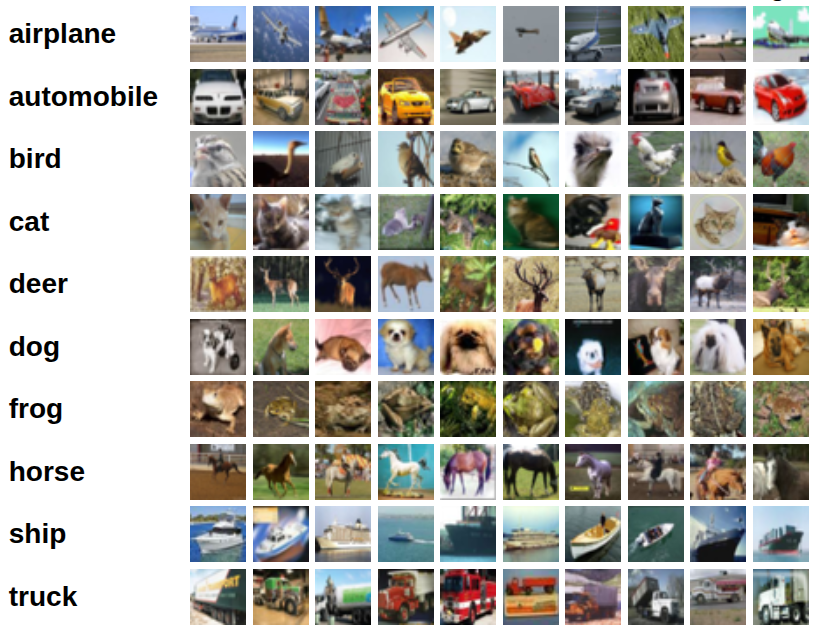
\includegraphics[width=0.9\linewidth]{cifar10.png}
      \caption{Sample images from CIFAR-10 dataset\footcite{krizhevsky2009}}
    \end{figure}
  \end{multicols}
\end{frame}

\begin{frame}{Model Architecture\vspace{-0.4em}}
    \begin{figure}
      \centering
      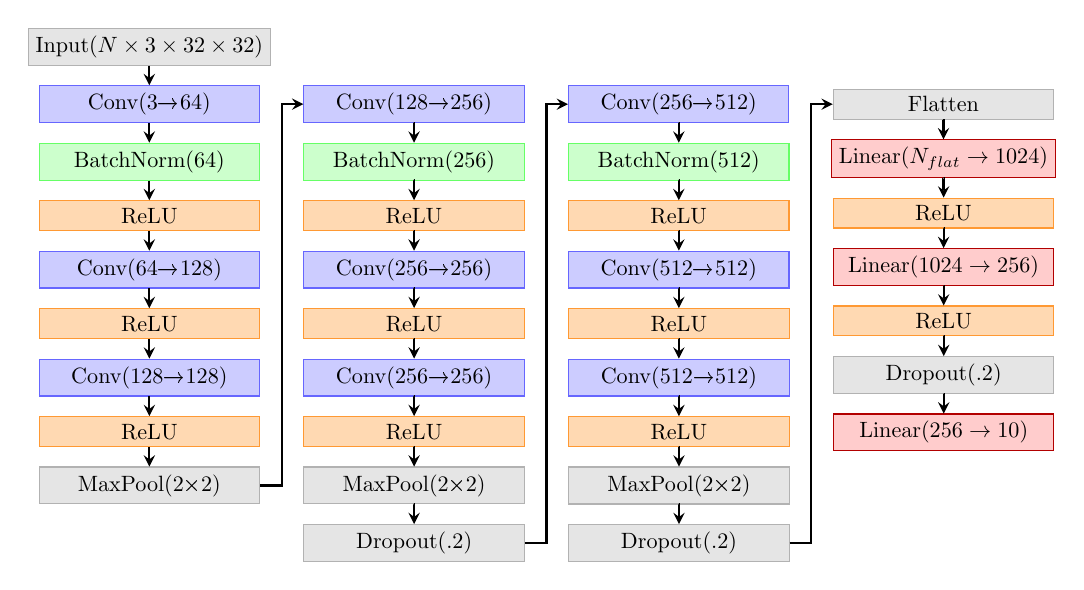
\begin{tikzpicture}[
        scale=0.1,
        nonparametric/.style={rectangle,draw=gray!60,fill=gray!20,minimum width=3.5cm,minimum height=0.4cm},
        conv/.style={rectangle,draw=blue!60,fill=blue!20,minimum width=3.5cm,minimum height=0.4cm},
        relu/.style={rectangle,draw=orange!80,fill=orange!30,minimum width=3.5cm,minimum height=0.4cm},
        bn/.style={rectangle,draw=green!60,fill=green!20,minimum width=3.5cm,minimum height=0.4cm},
        fc/.style={rectangle,draw=red!70!black,fill=red!20!,minimum width=3.5cm,minimum height=0.4cm},
        arrow/.style={->,thick},every node/.style={scale=0.8}
        ]

        \node (input)[nonparametric]{Input($N\times3\times32\times32$)};
        \def\distance{0.25cm}

        % --- Feature extractor ---
        \node (c1) [conv,below = \distance of input] {Conv(3→64)};
        \node (bn1) [bn,below = \distance of c1] {BatchNorm(64)};
        \node (r1) [relu,below = \distance of bn1] {ReLU};

        \node (c2) [conv,below = \distance of r1] {Conv(64→128)};
        \node (r2) [relu,below = \distance of c2] {ReLU};
        \node (c3) [conv,below = \distance of r2] {Conv(128→128)};
        \node (r3) [relu,below = \distance of c3] {ReLU};
        \node (p1) [nonparametric,below = \distance of r3] {MaxPool(2×2)};

        \node (c4) [conv,right = \distance+0.3cm of c1] {Conv(128→256)};
        \node (bn4) [bn,below = \distance of c4] {BatchNorm(256)};
        \node (r4) [relu,below = \distance of bn4] {ReLU};
        \node (c5) [conv,below = \distance of r4] {Conv(256→256)};
        \node (r5) [relu,below = \distance of c5] {ReLU};
        \node (c6) [conv,below = \distance of r5] {Conv(256→256)};
        \node (r6) [relu,below = \distance of c6]{ReLU};
        \node(p2)[nonparametric,below=\distance of r6]{MaxPool(2×2)};

        % dropout + next block
        \node(drp1)[nonparametric,below=\distance of p2]{Dropout(.2)};
        \node(c7)[conv ,right=\distance+0.3cm of c4]{Conv(256→512)};
        \node(bn7)[bn ,below=\distance of c7]{BatchNorm(512)};
        \node(r7)[relu ,below=\distance of bn7]{ReLU};
        \node(c8)[conv ,below=\distance of r7]{Conv(512→512)};
        \node(r8)[relu ,below=\distance of c8]{ReLU};
        \node(c9)[conv ,below=\distance of r8]{Conv(512→512)};
        \node(r9)[relu ,below=\distance of c9]{ReLU};
        \node(p3)[nonparametric ,below=\distance of r9]{MaxPool(2×2)};
        \node(drp2)[nonparametric ,below=\distance of p3]{Dropout(.2)}; 
        % --- classifier ---
        \node(flatten)[nonparametric ,right=\distance+0.3cm of c7]{Flatten};
        \node(fc11)[fc, below=\distance of flatten]{Linear($N_{flat}\to1024$)}; 
        \node(r10)[relu , below=\distance of fc11]{ReLU}; 
        \node(fc21)[fc , below=\distance of r10 ]{Linear($1024\to256$)}; 
        \node(r11)[relu , below=\distance of fc21 ]{ReLU}; 
        \node(drp3)[nonparametric , below=\distance of r11 ]{Dropout(.2)}; 
        \node(out)[fc , below=\distance of drp3 ]{Linear($256\to 10$)}; 

        % connections
        \foreach \a/\b in {
        input/c1,
        c1/bn1,
        bn1/r1,
        r1/c2,
        c2/r2,
        r2/c3,
        c3/r3,
        r3/p1,
        c4/bn4,
        bn4/r4,
        r4/c5,
        c5/r5,
        r5/c6,
        c6/r6,
        r6/p2,
        p2/drp1,
        c7/bn7,
        bn7/r7,
        r7/c8,
        c8/r8,
        r8/c9,
        c9/r9,
        r9/p3,
        p3/drp2,
        flatten/fc11,
        fc11/r10,
        r10/fc21,
        fc21/r11,
        r11/drp3,
        drp3/out}
        {
            \coordinate (\a\b) at ($ (\a)!0.5!(\b) $);
            \draw[->, thick, >=stealth] (\a.south) -| (\a\b) -| (\b);
            
        }
        \foreach \a/\b in{
        p1/c4,
        drp1/c7,
        drp2/flatten}
        {
            \coordinate (\a\b) at ($ (\a)!0.5!(\b) $);
            \draw[->, thick, >=stealth](\a)-|(\a\b)|-(\b);
        }
      \end{tikzpicture}
      \caption{CNN architecture inspired by AlexNet}
    \end{figure}
\end{frame}

\begin{frame}{Training setup}
  \begin{multicols}{2}
    \begin{itemize}
        \item \textbf{Framework:} PyTorch
        \item \textbf{Optimizer:} SGD with learning rate $0.01$, momentum $0.9$, weight decay $5\cdot10^{-4}$
        \item \textbf{Loss function:} Cross-Entropy Loss
        \item \textbf{Batch size:} 128
        \item \textbf{Epochs:} 100
        \item \textbf{Hardware:} NVIDIA GTX 3060, 12GB VRAM
        \item Logging with MLFlow\footnote{\url{https://mlflow.org/}}
        \item Model analysis with FiftyOne\footnote{\url{https://voxel51.com/fiftyone/}}
        \item[$\Rightarrow$] 88.3\% accuracy after 100 epochs
    \end{itemize}
    
    \vfill\null
    \columnbreak
    \begin{figure}
      \centering
      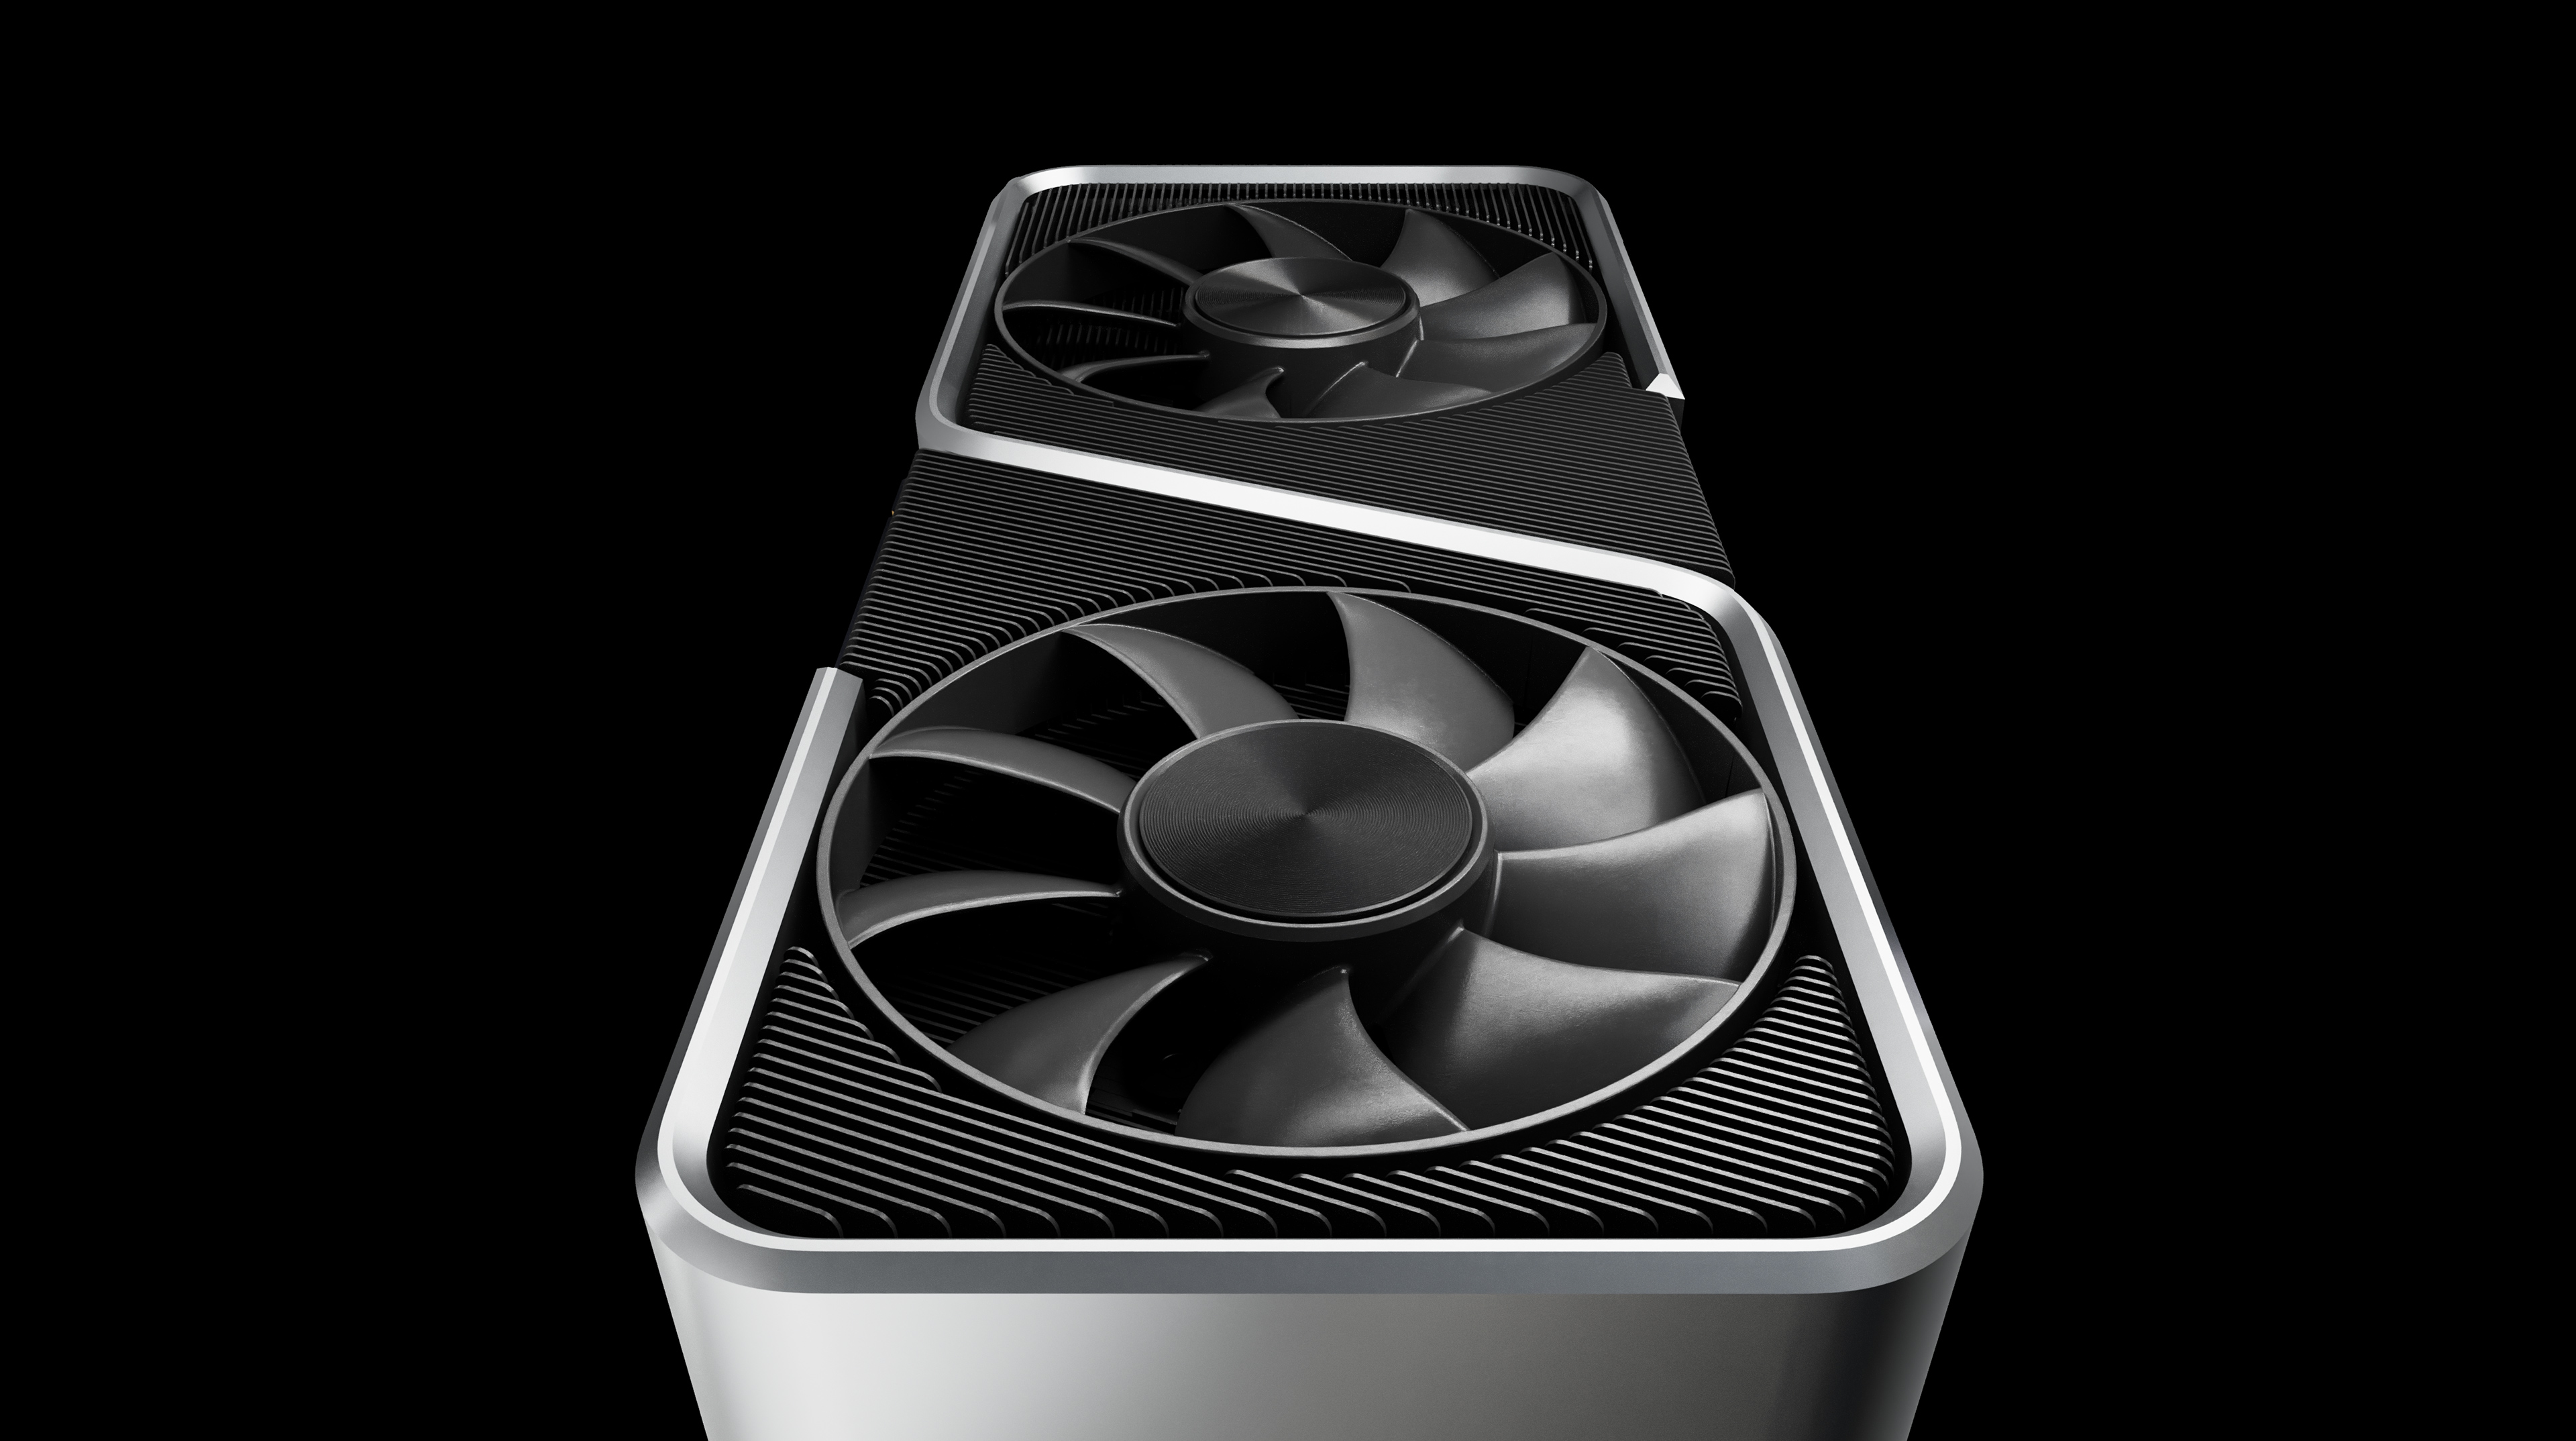
\includegraphics[width=0.9\linewidth]{graphics_card.png}
      \caption{NVIDIA GTX 3060\footnote{\url{https://www.nvidia.com/de-de/geforce/graphics-cards/30-series/rtx-3060-3060ti/}} used for training}
    \end{figure}
  \end{multicols}
\end{frame}

\begin{frame}{Data Augmentation \vspace{-1em}}
  \begin{multicols}{2}
    \begin{itemize}
      \item Color Jitter (brightness, contrast, saturation)
      \item Perspective Transform
      \item Random Horizontal Flip
    \end{itemize}
  \vfill\null
  \columnbreak
    \begin{itemize}
      \item[$\Rightarrow$] 92.5\% accuracy after 100 epochs with data augmentation
  \end{itemize}
  \end{multicols}
  \vskip-2em
  \begin{figure}
    \centering
    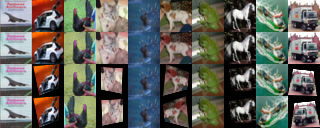
\includegraphics[width=0.8\linewidth]{augmented_images.png}
    \caption{Example of data augmentation techniques applied to a CIFAR-10 image}
  \end{figure}
\end{frame}

\begin{frame}{Training setup}
\begin{tikzpicture}[
  box/.style={rectangle, draw=black, minimum width=3cm, minimum height=1cm},
  arrow/.style={->, thick, >=stealth},
]
  \def\distance{1.1}

  \node (laptop) at (0,0) {\huge\faLaptop};
  \node (cloud)[above=3 of laptop] {\huge\faCloud};

  \node (python)[right=\distance of laptop, box] {\faPython Pycharm};
  \node (mlflow)[right=\distance of python, box] {\faServer mlflow};
  \node (port)[above=-1.6mm of mlflow] {\faDoorOpen};
  \node (portText)[above=0mm of port] {\small Port 5000};
  \node (fiftyone)[below=0.6 of mlflow, box] {\faServer \texttt{fiftyone}};
  \node (terminal)[right=\distance of mlflow, box] {\faTerminal Terminal};

  \node (github)[right=\distance of cloud, box] {\faGithub GitHub};
  \node (gpu)[above=3 of terminal, box] {\faMicrochip GPU Server};

  \draw[double,double distance=3mm, draw=green!50!black, thick] (terminal) + (0, 0.7) -- (gpu) node[midway, left, green!50!black, distance=2mm] {\faLock SSH\quad\ };

  \draw<2->[->, arrow] (python) -- (github) node[midway, right] {\texttt{git push}};
  \draw<3->[->, arrow] (github) -- (gpu) node[midway, above] {\texttt{git pull}};
  \draw<3->[->, transform canvas={xshift=0.2em}, arrow] (terminal) -- (gpu) node[midway, right] {control};
  \coordinate (logging_corner) at ($(terminal.north) + (0.0,0.19)$);
  \draw<4->[->,transform canvas={xshift=-0.2em}, draw=blue!50!black, arrow] (gpu) -- (logging_corner) |- (port) node[pos=0.75, above, blue!50!black] {logging};
  \draw<5->[->, arrow] (mlflow) -- (fiftyone) node[midway, right] {analyze best model};
\end{tikzpicture}
\end{frame}

\begin{frame}{Results}
  \begin{figure}[t!]
    \centering
    \begin{subfigure}{0.32\textwidth}
      \centering
      \begin{tikzpicture}
        \begin{axis}[
            width=1\linewidth,
            height=6cm,
            xlabel={Epochs},
            %ylabel={Accuracy},
            xmin=0, xmax=100,
            ymin=0, ymax=1,
            grid=both,
            grid style={line width=.1pt, draw=gray!10},
            major grid style={line width=.2pt,draw=gray!50},
            minor tick num=5,
            legend pos=south east,
            legend cell align={left},
            legend style={font=\scriptsize}
        ]
        \addplot[
            color=blue,
            mark=none,
            thick,
        ] table [x=step, y=value, col sep=comma] {data/vanilla_train.csv};
        \addlegendentry{Train Accuracy}
        \addplot[
            color=red,
            mark=none,
            thick,
        ] table [x=step, y=value, col sep=comma] {data/vanilla_val.csv};
        \addlegendentry{Test Accuracy}
        \end{axis}
      \end{tikzpicture}
      \caption{Accuracy in vanilla training}
    \end{subfigure}
    \hfill
    \begin{subfigure}{0.32\textwidth}
      \centering
      \begin{tikzpicture}
        \begin{axis}[
            width=1\linewidth,
            height=6cm,
            xlabel={Epochs},
            %ylabel={Accuracy},
            xmin=0, xmax=100,
            ymin=0, ymax=1,
            grid=both,
            grid style={line width=.1pt, draw=gray!10},
            major grid style={line width=.2pt,draw=gray!50},
            minor tick num=5,
            legend pos=south east,
            legend cell align={left},
            legend style={font=\scriptsize}
        ]
        \addplot[
            color=blue,
            mark=none,
            thick,
        ] table [x=step, y=value, col sep=comma] {data/aug_train.csv};
        \addlegendentry{Train Accuracy}
        \addplot[
            color=red,
            mark=none,
            thick,
        ] table [x=step, y=value, col sep=comma] {data/aug_val.csv};
        \addlegendentry{Test Accuracy}
        \end{axis}
      \end{tikzpicture}
      \caption{Accuracy with data augmentation}
    \end{subfigure}
    \hfill
    \begin{subfigure}{0.32\textwidth}
      \centering
      \begin{tikzpicture}
        \begin{axis}[
            width=1\linewidth,
            height=6cm,
            xlabel={Epochs},
            %ylabel={Accuracy},
            xmin=0, xmax=100,
            ymin=0, ymax=1,
            grid=both,
            grid style={line width=.1pt, draw=gray!10},
            major grid style={line width=.2pt,draw=gray!50},
            minor tick num=5,
            legend pos=south east,
            legend cell align={left},
            legend style={font=\scriptsize}
        ]
        \addplot[
            color=blue,
            mark=none,
            thick,
        ] table [x=step, y=value, col sep=comma] {data/sched_train.csv};
        \addlegendentry{Train Accuracy}
        \addplot[
            color=red,
            mark=none,
            thick,
        ] table [x=step, y=value, col sep=comma] {data/sched_val.csv};
        \addlegendentry{Test Accuracy}
        \end{axis}
      \end{tikzpicture}
      \caption{Accuracy with lr scheduling}
    \end{subfigure}
    \caption{Training performance}

  \end{figure}
\end{frame}

\begin{frame}[allowframebreaks]{References}
    \printbibliography
\end{frame}

\end{document}